The imaging and navigation layer consists of the Intel Realsense camera, ultrasonic sensors, and imaging software to produce navigation data to be sent to the drive system interface. The navigation data that will direct the crab drive system to follow a user as well as obstacle avoidance.

\begin{figure}[h!]
	\centering
 	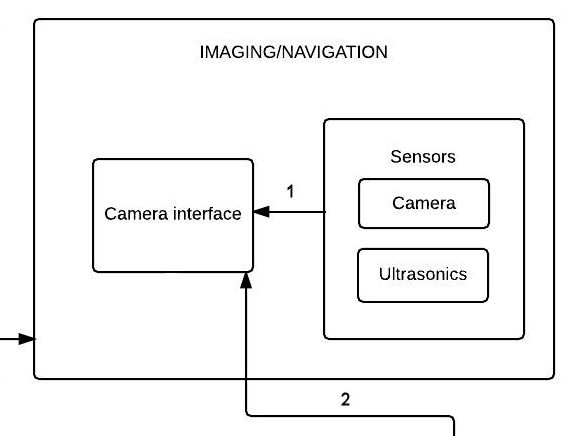
\includegraphics[width=0.60\textwidth]{images/imaging}
 \caption{Imaging and navigation layer}
\end{figure}

\subsection{Sensors Subsystem}
Sensors include the Intel RealSense camera and ultrasonic sensors. The RealSense will identify a user to follow and the ultrasonic sensors will be used for obstacle avoidance. The sensors will provide the necessary information to the camera interface needed to create navigation data.

\begin{figure}[h!]
	\centering
 	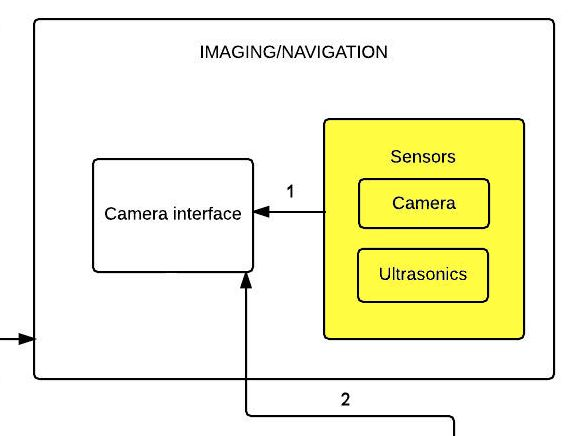
\includegraphics[width=0.60\textwidth]{images/imaging_sensors}
 \caption{Sensors subsystem}
\end{figure}

\subsubsection{Assumptions}
Assumptions made are as follows:
\begin{itemize}
	\item The user will be wearing a colored wristband that identifies them as the master.
	\item The user will stay in front of the Intel RealSense to avoid possible errors, such as the cart losing vision of its master.
\end{itemize}

\subsubsection{Responsibilities}
The sensor subsystem's responsibilities are as follows:
\begin{itemize}
	\item Process image and ultrasonic data in real time.
	\item Keep the designated master within the image frame.
	\item Gather accurate data to send to the camera interface.
\end{itemize}

\subsubsection{Subsystem Interfaces}

\begin {table}[H]
\caption {Sensors subsystem interfaces} 
\begin{center}
    \begin{tabular}{ | p{1cm} | p{6cm} | p{3cm} | p{3cm} |}
    \hline
    ID & Description & Inputs & Outputs \\ \hline
    \#1 & Send sensor data & \pbox{3cm}{Camera \\ Ultrasonics} & \pbox{3cm}{Camera interface}  \\ \hline
    \end{tabular}
\end{center}
\end{table}
\newline


\subsection{Camera Interface Subsystem}
The camera interface is responsible for taking the data received from sensors to calculate accurate navigation data to send to the crab drive's drive system interface. The navigation data will include required speed, direction needed, and cart position for collision avoidance.

\begin{figure}[h!]
	\centering
 	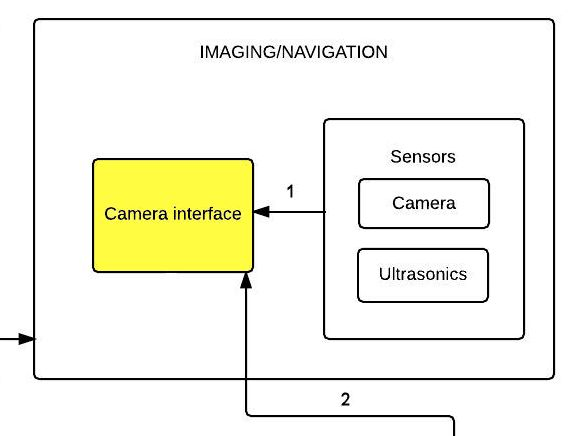
\includegraphics[width=0.60\textwidth]{images/imaging_camera}
 \caption{Camera interface subsystem}
\end{figure}

\subsubsection{Assumptions}
Assumptions made are as follows:
\begin{itemize}
	\item Accurate data is being sent from the sensors.
	\item The camera interface will be able to communicate with the drive system interface.
\end{itemize}

\subsubsection{Responsibilities}
The camera interface subsystem's responsibilities are as follows:
\begin{itemize}
	\item Calculate and process navigation data.
	\item Communicate necessary information to the drive system interface.
\end{itemize}

\subsubsection{Subsystem Interfaces}

\begin {table}[H]
\caption {Camera interface subsystem interfaces} 
\begin{center}
    \begin{tabular}{ | p{1cm} | p{6cm} | p{3cm} | p{3cm} |}
    \hline
    ID & Description & Inputs & Outputs \\ \hline
    \#2 & Calculate navigation data & \pbox{3cm}{Sensors} & \pbox{3cm}{Drive system interface}  \\ \hline
    \end{tabular}
\end{center}
\end{table}
